\chapter{Modellierung und Entwurf}
\label{cha:Modellierung und Entwurf}

In diesem Kapitel werden die funktionalen Anforderungen aus dem Abschnitt \ref{sec:anforderungsdefinition} spezifiziert. Modelle für die einzelnen funktionalen Anforderungen sollen entwickelt werden. Die Modelle veranschaulichen das geforderte funktionale Verhalten der Software. Voraussetzung für die Entwicklung der Modelle ist die Konkretisierung der funktionalen Anforderungen. Diese Konkretisierung beinhaltet die Festlegung der Bestandteile die für eine Implementierung der funktionalen Anforderung benötigt werden. Ziel des Kapitels ist es, die wichtigsten Bestandteile einer funktionalen Anwendung herauszubilden, dieses Bestandteile zu definieren und zu veranschaulichen. 

\section{Tic Tac Toe}
\label{sec:Tic Tac Toe}

Das klassische Tic Tac Toe ist ein Spiel, welches mit genau zwei Spielern gespielt wird. Jeder dieser Spieler setzt abwechselnd entweder ein Kreuz oder einen Kreis. Während eines gesamten Spiels darf ein Spieler nur Kreuze setzen und der andere Spieler nur Kreise. Wir können uns die Kreuze und Kreise als Spielfiguren vorstellen, die sobald sie auf das Spielfeld gesetzt wurden, nicht mehr verändert oder verschoben werden können. Das Spielfeld ist eine drei mal drei große Matrix, also können maximal neun Spielfiguren in diese Matrix gesetzt werden. Im ersten Spielzug stehen dem Spieler neun mögliche Positionen zur Verfügung. Die Anzahl der möglichen Positionen reduziert sich jede Runde um eins. Folglich ist die maximale Länge einer Spielzugsequenz, bei einem drei mal drei Spielfeld, neun. Maximal deshalb, weil das Spiel auch vor der neunten Runde bereits entschieden sein kann. \\

\subsection{Spielregeln}
\label{subsec:Spielregeln}

Ziel des Spiels ist es vier Kreuze oder vier Kreise in einer bestimmten Position anzuordnen. Es wird davon ausgegangen, dass zwei Spieler Alice und Bob existieren und gegeneinander Tic Tac Toe spielen. Alice setzt ausschließlich Kreuze und Bob ausschließlich Kreise. Wir gewähren Alice in unseren Beispielen immer den ersten Zug. Es existieren drei unterschiedliche Anordnungen von Spielfiguren, die das Spiel beenden und einen Sieg herbeiführen. Gewinnt ein Spieler mit einer Siegesanordnung seiner Spielfiguren, dann verliert der andere Spieler dadurch automatisch in gleicher Höhe (Nullsummenspiel). \\

\begin{figure}[!htbp]
  \centering
  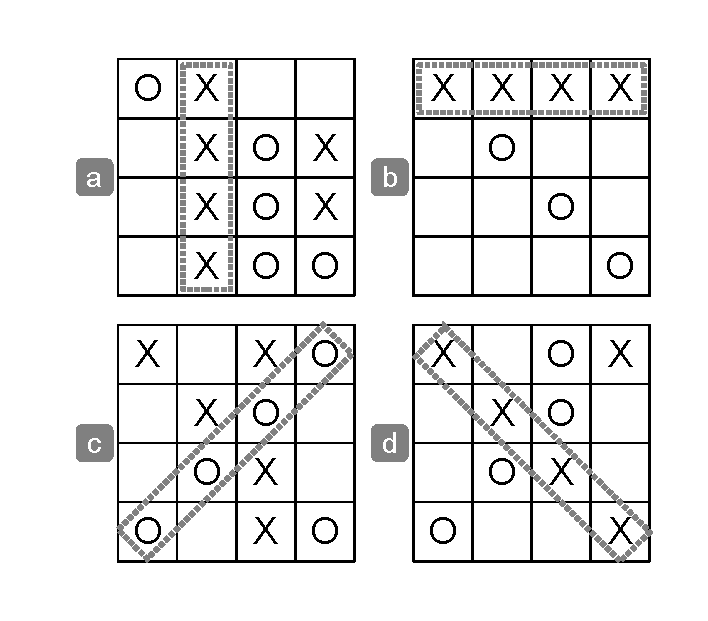
\includegraphics[scale = 1]{inhalt/abbildungen/siegesbedingungen_tictactoe.pdf}
  \caption{Veranschaulichung der vertikalen (a), horizontalen (b) und diagonalen (c, d) Siegesbedingung.}
  \label{fig:siegesbedingungen_tictactoe}
\end{figure}

In Abbildung \ref{fig:siegesbedingungen_tictactoe} a, gewinnt Alice knapp gegen Bob mit einer ununterbrochenen vertikalen Anordnung ihrer Spielfiguren. Bob hätte fast eine diagonale Reihe aus Kreisen verbunden, diese wurde jedoch von Alice mit einer Spielfigur geblockt. Zudem hätte Bob auch fast eine vertikale Spalte ohne Unterbrechungen vervollständigt. Eine horizontale Siegesanordnung entsteht, wenn vier Spielfiguren eines Spielers in einer horizontalen Zeile angeordnet sind. Alice gewinnt das zweite Spiel gegen Bob durch eine horizontale Siegesanordnung (siehe Abbildung \ref{fig:siegesbedingungen_tictactoe} b). In jeder Spalte des Spielfeldes ist genau eine vertikale und in jeder Zeile des Spielfeldes ist genau eine horizontale Siegesanordnung möglich. Die dritte und letzte Anordnungsvariante der Spielfiguren, welche zu einem Sieg eines Spielers führt, ist die diagonale Verbindung von vier Spielfiguren eines Spielers. In Abbildung  \ref{fig:siegesbedingungen_tictactoe} c, gewinnt Bob mit einer diagonalen Anordnung von vier Spielfiguren ohne Unterbrechung einer gegnerischen Spielfigur. Alice gewinnt ebenfalls eine Party, durch einen diagonale Siegesanordnung (Abbildung \ref{fig:siegesbedingungen_tictactoe} d). Eine Party wird, in diesem Kontext, als ein abgeschlossenes Spiel, mit anschließendem Ergebnis, verstanden. \\

Bei einem vier mal vier Spielfeld existieren vier vertikale, vier horizontale und zwei diagonale Anordnungen der Spielfiguren, welche einen Sieg herbeiführen würden. Insgesamt zehn verschiedene Siegesanordnungen für beide Spieler. Was passiert jedoch, wenn keine der zehn möglichen Siegesanordnungen auftritt, dann gewinnt beziehungsweise verliert keiner der beiden Spieler und es entsteht ein Unentschieden. Sind die beiden Kontrahenten gleich gut, erfahren oder verwenden die selben Strategien, dann tritt ein Unentschieden möglicherweise öfter oder andauernd ein.

\subsection{Suchbaum}

\begin{figure}[!htbp]
  \centering
  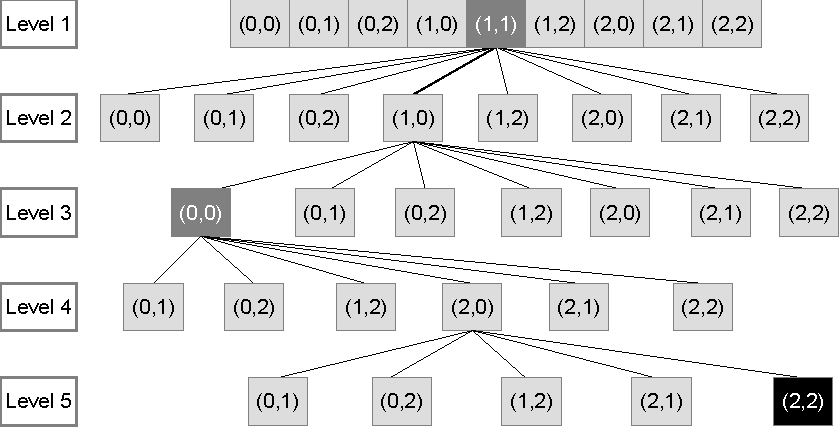
\includegraphics[scale = 1]{inhalt/abbildungen/suchbaum_drei_mal_drei_tictactoe.pdf}
  \caption{TicTacToe Spielbaum, eines drei mal drei Spielfeldes, der in Level fünf terminiert.}
  \label{fig:drei_mal_drei_tictactoe_spielbaum}
\end{figure}

Ein Suchbaum für ein drei mal drei Spielfeld, hat maximal eine Tiefe (Level) von neun. Der Verzweigungsfaktor im ersten Level ist äquivalent zur maximalen Tiefe des Suchbaums. Für jedes weitere Level reduziert sich der Verzweigungsfaktor um eins. In Level eins ist der Verzweigungsfaktor gleich neun, in Level fünf ist er gleich fünf und in Level neun ist er gleich  eins. Der Verzweigungsfaktor reduziert sich deshalb in jedem Spielzug, weil in jedem Spielzug eine Position mit einer Spielfigur besetzt wird und eine bereits besetzte Position darf nicht erneut besetzt werden. Der Sieg mit der kürzesten Spielzugsequenz ist nach fünf Spielzügen, für den beginnenden Spieler, zu erreichen. Bob der erst als zweites seinen Spielzug ausführen darf, kann erst ab einer Spielzugsequenz der Länge sechs gewinnen. Abbildung \ref{fig:drei_mal_drei_tictactoe_spielbaum} zeigt einen schwarz markierten terminierenden Endzustand (2,2) des Spielbaums in Level fünf. Alice erreicht diesen Endzustand, weil sie ihren Spielstein in Zeile zwei und Spalte zwei setzt. Die terminierenden Endzustände des Spielbaumes werden allgemein als Blattknoten bezeichnet. Ein Blattknoten charakterisiert, dass es keine weiteren Verzweigungen oder Knoten unterhalb dieses Blattknotens geben darf. \todo{Ist jeder Blattknoten ein Terminierender Endzustand?} Es gibt zwei Möglichkeiten für das erreichen eines Blattknotens(Bedingung der Terminierung):

\begin{enumerate}
\item Eine Siegesanordnung ist entstanden.
\item Alle möglichen Positionen des Spielfeldes sind besetzt und es wurde keine Siegesanordnung erreicht.
\end{enumerate}

In Level fünf bis Level neun können terminierende Endzustände auftreten, das heißt Alice kann in Level fünf, Level sieben und in Level neun eine Siegesformation erreichen. Bob hingegen kann in Level sechs und Level acht eine Siegesanordnung erhalten. Theoretisch fehlt Bob, dem Spieler der als zweites beginnt, ein Zug gegenüber dem zu erst beginnenden Spieler. Tritt ein terminierender Endzustand von Level fünf bis Level acht auf, dann wurde dieser Endzustand immer durch das erreichen einer Siegesanordnung hervorgerufen, sprich durch die 1. Bedingung der Terminierung. Ein Blattknoten in Level neun kann durch die 1. und 2. Bedingung der Terminierung entstehen, das heißt entweder ist das Spielfeld voll besetzt und es wurde keine Siegesanordnung gefunden oder das Spielfeld ist voll besetzt und es wurde eine Siegesanforderung gefunden. Folglich besteht Level neun ausschließlich aus Blattknoten. \\

5 * 8 * (3 * 3)
40 terminierende Endzustände

Wie viele verschiedene Zustände kann ein drei mal drei Tic Tac Toe Spielfeld haben?
Eine beliebige regelkonforme Anordnung von Spielsteinen auf dem Tic Tac Toe Spielfeld bezeichnen wir als einen Zustand $s_1$. Eine Menge die alle möglichen Zustände s enthält bezeichnen wir als die Menge S. Somit gilt $s_1, s_2 ... s_x \in S$. Der gesamte Spielbaum eines drei mal drei Tic Tac Toe Spielfeldes (Spielbaum ähnelt Abbildung \ref{fig:drei_mal_drei_tictactoe_spielbaum}) hat
 
\begin{equation}
\prod_{i=1}^{9} 9 - (i - 1) = 9 \times 8 \times 7 \times 6 \times 5 \times 4 \times 3 \times 2 \times 1 = 362880
\end{equation}

Blattkonten. In dieser Rechnung sind keine Positionsredundanzen und terminierende Endzustände berücksichtigt.
 

\begin{equation}
\prod_{i=0}^{5 - 1} 9 - i = 9 \times 8 \times 7 \times 6 \times 5 = 15120
\end{equation}

Um die Anzahl der möglichen Spielzüge zu erhöhen und um die mittlere unfaire Position in einem drei mal drei Spielfeld zu entfernen, wird das Spielfeld des klassischen Tic Tac Toe auf eine vier mal vier Matrix erweitert.

\subsection{Strategie}

\myparagraph{Spielfeldsymmetrie}

\begin{figure}[!htbp]
  \centering
  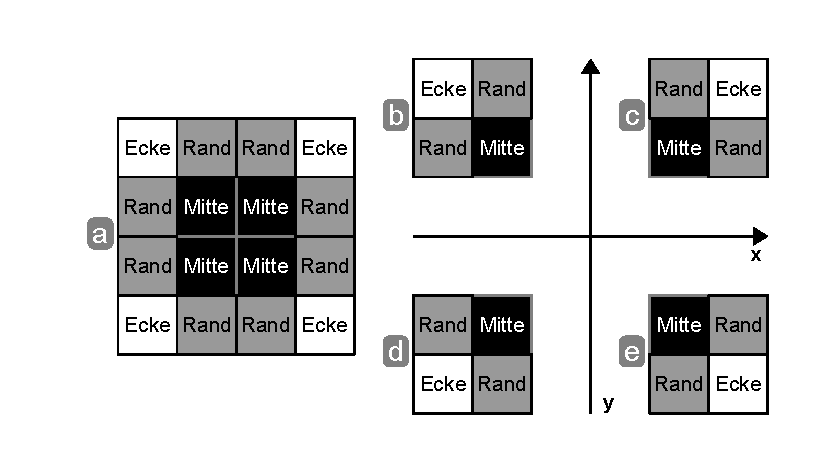
\includegraphics[scale = 1]{inhalt/abbildungen/symmetrie_tictactoe_spielfeld.pdf}
  \caption{Symmetrie Eigenschaften des vier mal vier Tic Tac Toe Spielfelds.}
  \label{fig:symmetrie_tictactoe_spielfeld}
\end{figure}

\myparagraph{Kontrolliere die Mitte}

\begin{figure}[!htbp]
  \centering
  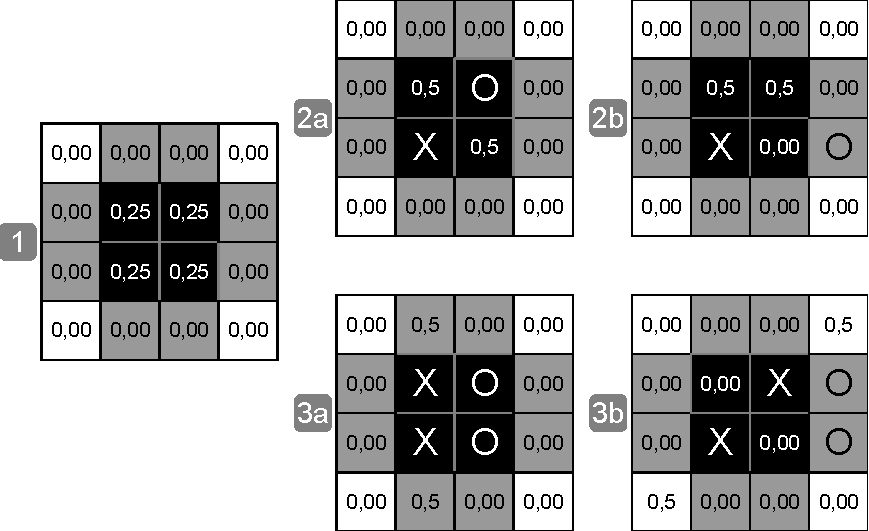
\includegraphics[scale = 0.8]{inhalt/abbildungen/kontrolliere_die_mitte.pdf}
  \caption{Strategie um die Mitte zu kontrollieren.}
  \label{fig:kontrolliere_die_mitte}
\end{figure}

\myparagraph{Verteidigung ist der beste Angriff}

\begin{figure}[!htbp]
  \centering
  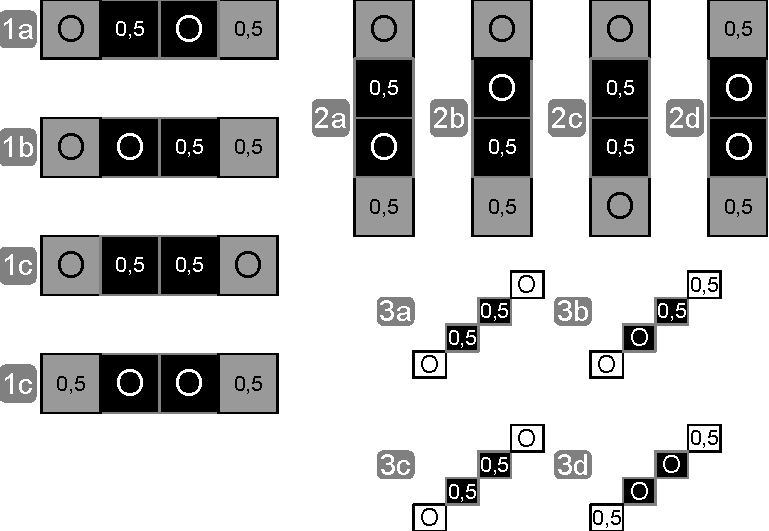
\includegraphics[scale = 0.8]{inhalt/abbildungen/verteidigung_ist_angriff.pdf}
  \caption{TicTacToe Spielzustände in denen Alice dringend verteidigen sollte und Bob angreifen kann.}
  \label{fig:verteidigung_ist_angriff}
\end{figure}

\subsection{Benutzerschnittstellen}

Alice kann ihre Kreuze auf das Spielfeld setzen, indem sie ein, vorher vom Spiel definiertes, Zahlentupel über die Tastatur eingibt. Welche Zahlentupel ein Kreuz an welche Stelle setzt ist in Abbildung \ref{fig:kreiseUndKreuzeSetzen} definiert. Sollte Alice keines der erlaubten Zahlentupel eingeben, dann wird sie darauf hingewiesen, welche Steuerungsmöglichkeiten ihr, zum setzen der Spielfiguren, zur Verfügung stehen.

\begin{figure}[!htbp]
  \centering
  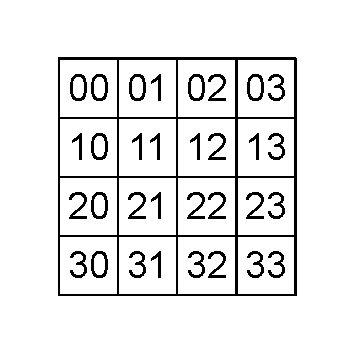
\includegraphics[scale = 1]{inhalt/abbildungen/vier_mal_vier_matrix.pdf}
  \caption{Tic Tac Toe Spielfiguren setzen}
  \label{fig:kreiseUndKreuzeSetzen}
\end{figure}

\section{Reversi}
\myparagraph{Spielprinzipien}
\myparagraph{Spielregeln}
\myparagraph{Benutzerschnittstellen}

\section{Lernverfahren}
\label{sec:lernverfahren}
\subsection{Analyse und Auswahl der lernfähigen Algorithmen}

\subsection{Anwendung der Algorithmen auf Computerspiele}

\subsection{Konzeptuelles Training der Algorithmen}

\subsection{Persistenz der Trainingsdaten}